\part[The Java Ecosystem]{The Java Ecosystem}
\section{Metal programming}

\begin{frame}{Once upon a time\ldots}
\visible<2->{in the land of computers there were 10101110010101101\ldots\\}
\visible<3->{then assemblers came along\ldots\\}
\visible<4->{followed by compilers\ldots\\}
\visible<5->{and they lived happily ever after\ldots \visible<6->{\alert{NOT!}}}
\end{frame}

\begin{frame}[fragile]{Portability}
\begin{alertblock}{Platform Dependency}
\begin{lstlisting}
for(os <- List("linux", "mac", "windows"))
  println("If you compile a C program under " + os
            + "you can run it only on " + os + ".")
\end{lstlisting}
\end{alertblock}
\pause
Sometimes a recompilation is not sufficient. \alert{The code} has to be adapted!
\pause
\begin{block}{Platform Independency}
Write Once, Run Anywhere.
\end{block}
\end{frame}

\pictureframe{Problem - Unmanaged code}{resources/PlatformDependency.pdf}

\begin{frame}{Problem - Unmanaged code 2}
\begin{block}{Why is unmanaged code a problem?}
\begin{enumerate}
  \pause
  \item portability issues
  \pause
  \item low level hazards like buffer overflows, segmentation faults etc.
\end{enumerate}
\end{block}
\pause
\begin{alertblock}{The problem, programming language designers are trying to
solve:} Software development is not about programming the hardware, it is about
abstracting over the hardware!
\end{alertblock}
\end{frame}

\pictureframe{Solution - Managed code}{resources/PlatformIndependency.pdf}

\begin{frame}{Solution - Managed code 2}
\begin{block}{Why is managed code a solution?}
\begin{enumerate}
  \pause
  \item portability issues are being taken care by VM vendors.
  \pause
  \item low level hazards like buffer overflows, segmentation faults etc. are
  being handled by the VM.
  \pause
  \item programs as-well as programming languages are changing every second;
  platforms are fairly stable!
\end{enumerate}
\end{block}
\pause
\begin{block}{Wind of Change}
\begin{itemize}
  \item it is \textcolor{blue}{feasible} to change a program.
  \item it is \textcolor{orange}{hard} to change a programming language.
  \item it is \textcolor{red}{very hard} to change a platform, but platforms are
  not required to be frequently changed.
\end{itemize}
\end{block}
\end{frame}

\begin{frame}{Virtual Machines}
\begin{block}{What is an Operating System?}
An operating system is an abstraction over a hardware \highlight{machine}.
\end{block}
\pause
\begin{block}{What is a Virtual Machine?}
A \highlight{virtual} machine is an abstraction over an operating system.
\end{block}
\pause
\begin{exampleblock}{Well-known VMs}
\begin{description}
  \item[Java] Java Virtual Machine (JVM)
  \item[.Net] Common Language Runtime (CLR)
  \item[Android] Dalvik virtual machine
  \item
  and
  \link{http://www.en.wikipedia.org/wiki/Virtual_machine\#List_of_virtual_machine_software}{many more}
\end{description}
\end{exampleblock}
\end{frame}

\begin{frame}{Managed Programming Languages}
\begin{block}{JVM - runs everywhere}
\begin{description}[<+->]
	\item[\link{http://en.wikipedia.org/wiki/Java_\%28programming_language\%29}{Java}]
	Statically typed OO language
	\item[\link{http://en.wikipedia.org/wiki/Scala_programming_language}{Scala}]
	Statically typed OO \& FP language
	\item[\link{http://en.wikipedia.org/wiki/Clojure}{Clojure}] Dynamically
	typed FP language
	(\link{http://en.wikipedia.org/wiki/Lisp_\%28programming_language\%29}{Lisp}
	dialect)
	\item[\link{http://en.wikipedia.org/wiki/Groovy_\%28programming_language\%29}{Groovy}]
	Dynamically typed scripting language
	\item and \link{http://en.wikipedia.org/wiki/List_of_JVM_languages}{many
	more}
\end{description}
\end{block}
\begin{block}{CLR - runs only on Windows}
\begin{description}[<+->]
	\item[\link{http://en.wikipedia.org/wiki/C_Sharp_\%28programming_language\%29}{C\#}]
	Statically typed OO \& FP language
	\item[\link{http://en.wikipedia.org/wiki/Visual_Basic_.NET}{VB}] Statically
	typed OO language
	\item[\link{http://en.wikipedia.org/wiki/F_Sharp_\%28programming_language\%29}{F\#}]
	Statically typed FP language
	\item
	and
	\link{http://en.wikipedia.org/wiki/List_of_CLI_languages\#CLI_languages}{many more}
\end{description}
\end{block}
\end{frame}

\begin{frame}{Managed Programming Languages 2}
\begin{block}{Dalvik - designed for Android}
Java is officially supported. Every JVM language should theoretically
work. \highlight{Scala}
works.
\link{http://stackoverflow.com/questions/1994703/which-programming-languages-can-i-use-on-android-dalvik}{Few others} work as-well.
\end{block}
\end{frame}

\begin{frame}{JVM - People's Choice}
\begin{center}

\includegraphics[scale=0.25]{resources/JVM.png}
\end{center}
The code is \alert{not} compiled to \highlight{binary}.\\
The code is compiled to the so called \highlight{bytecode}.\\
The \highlight{JVM} is a software component, which runs the
\highlight{bytecode}.\\
A JVM implementation exists for almost \highlight{every platform}.\\
\highlight{Java} is the most used language on the \highlight{JVM}.\\
The most used \highlight{Java} compiler is called \highlight{javac}. 
\end{frame}

\pictureframe{What language should we use for the JVM?}{resources/Language.pdf}
\pictureframe{Can we reuse the java compiler for this
language?}{resources/Compiler.pdf}

\section{A History Lesson\ldots}
\begin{frame}{The Java Time Line}
\begin{block}{1996}
\highlight{Java 1.0} designed by James Gosling
\end{block}
\begin{center}
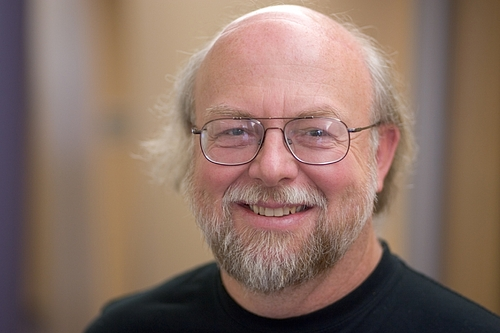
\includegraphics[scale=0.4]{resources/JamesGosling.jpg}
\end{center}
\end{frame}

\begin{frame}{The Java Time Line 2}
\begin{block}{1997}
Marin Odersky and Philip Wadler start working on \highlight{Pizza}.
\begin{itemize}
\item Pizza is Java + extensions (generics, higher-order functions, etc.)
\item Pizza compiler translates Pizza \highlight{source} code \highlight{to}
Java \highlight{source} code so that the Java compiler can translate it to bytecode.
\end{itemize}
\end{block}
\begin{columns}
	\column{.5\textwidth}
	\begin{center}
	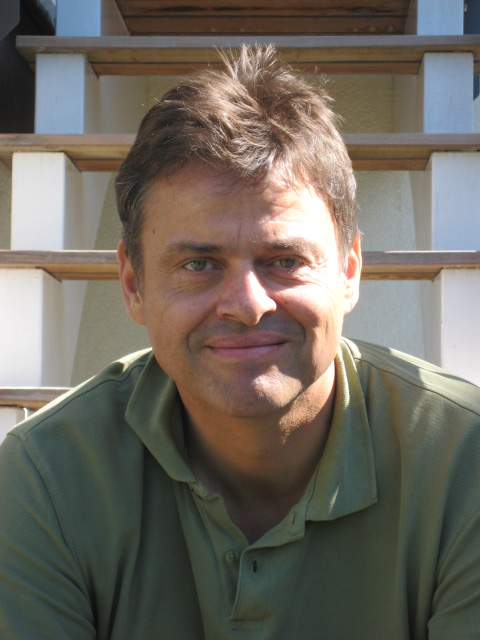
\includegraphics[width=0.5\textwidth]{resources/MartinOdersky.jpg}
	\end{center}
	\column{.5\textwidth}
	\begin{center}
	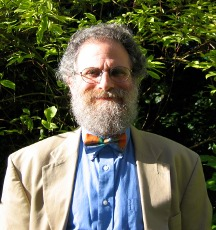
\includegraphics[width=0.5\textwidth]{resources/PhilipWadler.jpg}
	\end{center}
\end{columns}
\end{frame}

\begin{frame}{The Java Time Line 3}
\begin{block}{1998}
Bracha, Odersky, Stoutamire and Wadler design \highlight{Generic Java (GJ)} for
JavaSoft (later known as Sun Microsystems).
\begin{itemize}
\item GJ compiler translates Generic Java (Java + parts of Pizza) source code
directly to bytecode.
\item GJ adopts only generics from Pizza.
\end{itemize}
\end{block}
\begin{center}
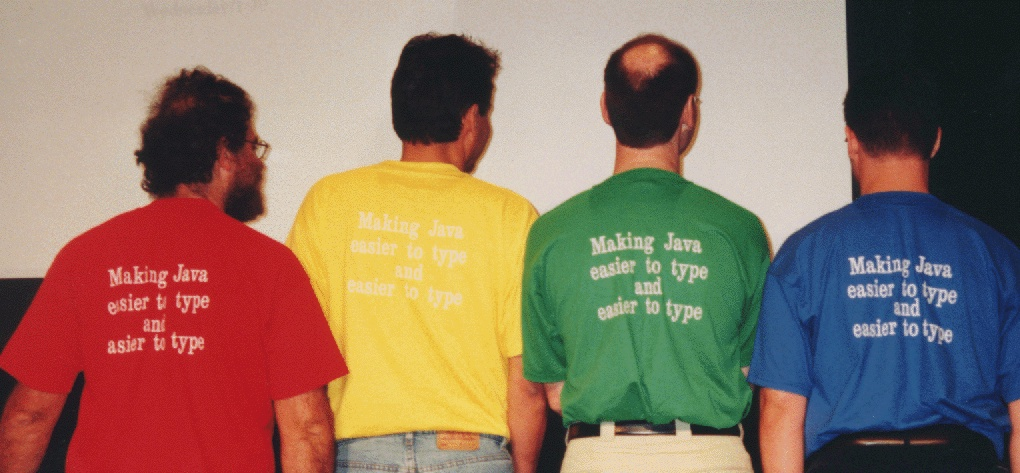
\includegraphics[width=0.7\textwidth]{resources/GJBack.jpg}
\end{center}
\end{frame}

\begin{frame}{The Java Time Line 4}
\begin{block}{2000}
GJ compiler becomes \highlight{javac} in JDK 1.3
\begin{itemize}
\item the new javac is more stable, correct and even performs better.
\item javac (GJ compiler) still compiles Java (\alert{not} GJ) to bytecode.
\end{itemize}
\end{block}
\pause
\begin{block}{2004}
Sun Microsystems releases \highlight{Java 1.5}
\begin{itemize}
\item generics from GJ finally make it to Java.
\end{itemize}
\end{block}
\pause
\begin{block}{2005-2010}
\highlight{Java 1.6}
\begin{itemize}
\item Java alternatives appear every day
\end{itemize}
\end{block}
\pause
\begin{block}{2011-present}
\highlight{Java 1.7}
\end{block}
\end{frame}

\begin{frame}{Meanwhile\ldots}
A long time ago in a galaxy far, far away....
\begin{block}{Mid-1980s}
A lot of research around functional programming languages. ML, OCaml, Miranda,
Lisp dialects like Scheme.
\begin{itemize}
  \item features like \highlight{type inference}, \highlight{lazy evaluation}
  and \highlight{higher-ranked types}.
\end{itemize}
\end{block}
\pause
\begin{block}{1987-1999}
Development of \highlight{Haskell} by Simon Peyton-Jones.
\begin{itemize}
  \item a \highlight{pure}, lazy, functional language with lots of new features
  \item advanced type system
  \item \highlight{Martin Odersky} contributes work on higher-ranked types to
  the \highlight{Glasgow Haskell Compiler}.
\end{itemize}
\end{block}
\end{frame}

\begin{frame}{Meanwhile\ldots}
\begin{center}
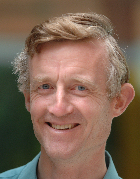
\includegraphics[width=0.2\textwidth]{resources/SimonPeytonJones.jpg}
\end{center}
\begin{block}{1999-2001}
Martin Odersky works on \highlight{Funnel} language at EPFL in Switzerland
\begin{itemize}
  \item basic principles, combines FP and Petri nets
  \item allows imperative, concurrent and OO programming
  \item compiles to JVM bytecode
  \item \alert{easy for academic folks, but too heavy for the industry}
\end{itemize}
\end{block}
\end{frame}

\begin{frame}{The Scala Time Line}
\begin{block}{2004}
\highlight{Scala} - The fresh start on Funnel
\begin{itemize}
  \item combines OO and FP
  \item static, but inferred typing
  \item features from Java and Pizza
\end{itemize}
\end{block}
\pause
\begin{block}{2008-2010}
Scala 2.x - 2.7x
\begin{itemize}
  \item Twitter takes Scala for a spin, and brings it into the Spotlight
  \item features from Haskell
  \item fine-grained qualification of access modifiers
  \item cutting edge features like \highlight{extractor objects} or
  \highlight{abstract types}
\end{itemize}
\end{block}
\end{frame}

\begin{frame}{The Scala Time Line 2}
\begin{block}{2011}
Scala 2.8x
\begin{itemize}
  \item complete rework of the collections framework
  \item The Typesafe company - commercial support for Scala
  \item Serious attention from the industry
\end{itemize}
Scala 2.9x
\begin{itemize}
  \item parallel collections
  \item own build tool - \highlight{Simple Build Tool (SBT)}
  \item better IDE and docs
\end{itemize}
\end{block}
\pause
\begin{block}{2012-present}
Scala 2.10x (in development at the moment)
\begin{itemize}
  \item new reflection framework
  \item dynamic typing (similar to C\# 4)
\end{itemize}
\end{block}
\end{frame}

\pictureframe{Scala - People's Choice}{resources/Scala.pdf}

\begin{frame}{Why should I learn Scala?}
\begin{block}{The Academic Point of View}
\begin{itemize}
  \item Cutting Edge language
  \item Pure OO language
  \item FP features
  \item Very advanced type system
  \item Joy
  \item You should learn a new programming language once in a year ;)
\end{itemize}
\end{block}
\end{frame}

\begin{frame}{Why should I learn Scala?}
\begin{block}{The Industrial Point of View}
\begin{itemize}
  \item OO language
  \item Makes you more productive
  \item Provides a worthy alternative for solving concurrency problems
  \item Seamless interoperability with Java
  \item Lots of Scala jobs out there!
\end{itemize}
\end{block}
\end{frame}

\pictureframe{Scala in the Industry}{resources/ScalaIndustry.pdf}

\begin{frame}{Java is not going to be here forever}
\begin{center}
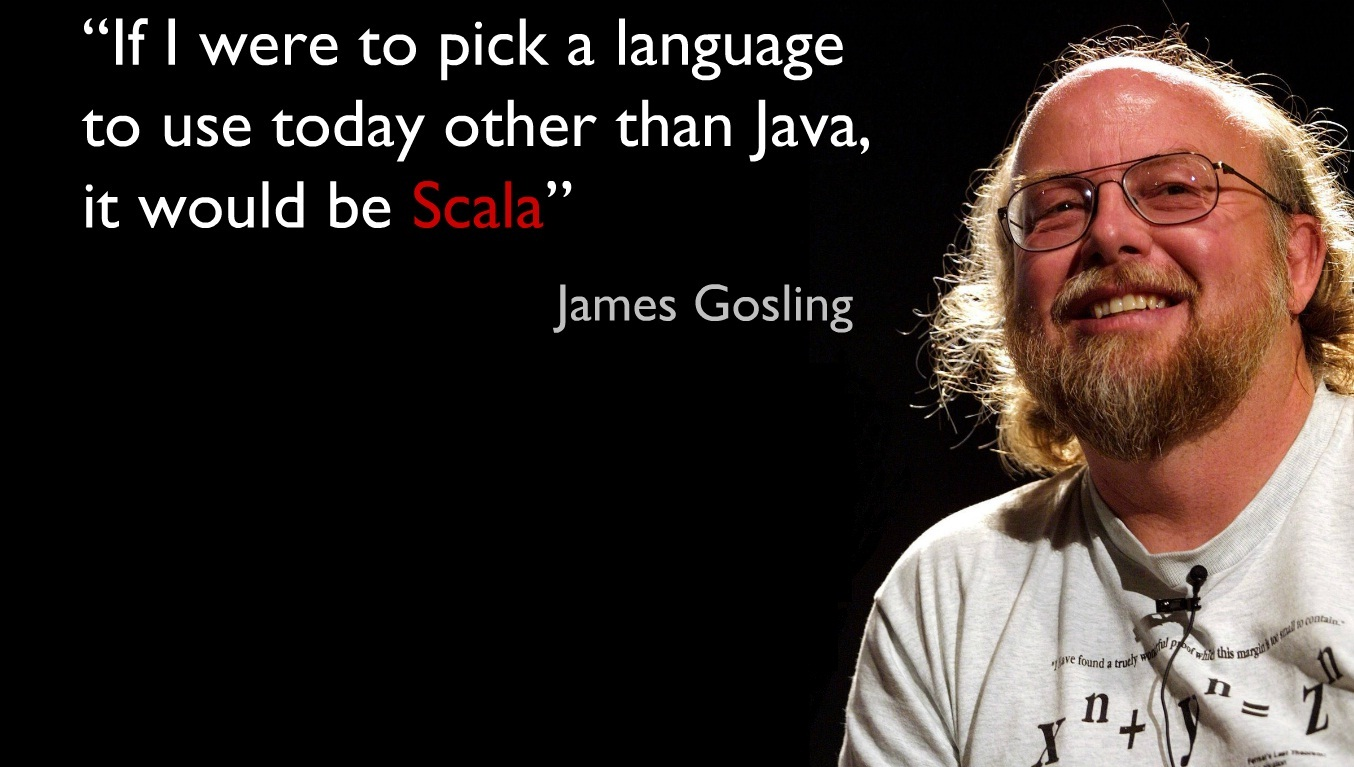
\includegraphics[scale=0.3]{resources/JamesGoslingScala.jpg}
\end{center}
\end{frame}

\begin{frame}{Java is not going to be here forever}
\begin{center}
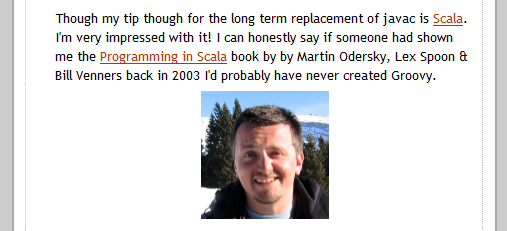
\includegraphics[scale=0.8]{resources/JamesStrachanScala.png}\\
James Strachan - designer of Groovy
\end{center}
\end{frame}

\begin{frame}{Summary}
\begin{itemize}
  \item \highlight{JVM} is a great platform
  \item \highlight{Java} is getting old
  \item \highlight{Scala} seems to be a great language
  \item Scala's \highlight{interoperability} with Java is seamless
  \item Scala combines \highlight{OO} with \highlight{FP}
  \item Scala is accepted in the \highlight{industry}
\end{itemize}
\end{frame}







